
\chapter{Return-oriented Programming ROP}
ROP è una tipologia di attacco a basso livello, assembly. Quando si compila un codice, viene caricata in quasi tutti i programmi Unix anche la libreria standard \textbf{libc}, la quale contiene delle routine utili per un attaccante. Per l'attacco vengono utilizzate solo piccole sequenze di codice, esse sono lunghe solo due o tre istruzioni (\textbf{gadget}). Alcune di esse sono presenti in \textbf{libc} come risultato delle scelte fatte dal compilatore durante la generazione del codice.

\section{Funzionamento dell'attacco}
La ROP è una tecnica simile all'arc injection, ma invece di ritornare alle funzioni, il codice di exploit ritorna a sequenze di istruzioni seguite da un return (\textbf{ret}).
Ogni sequenza di istruzioni utile è chiamata \textbf{gadget},
ognuno di essi specifica determinati valori da inserire nello stack che permettono di usare queste sequenza di istruzioni.
Essi sono delle istruzioni come load, add o jump. Questa tenica permette all'attaccante di eseguire codice in presenza di difese di sicurezza
come \textit{executable space protection}
\footnote{ Nella sicurezza del computer, la protezione dello spazio eseguibile contrassegna le regioni di memoria come non eseguibili,
    in modo tale che un tentativo di eseguire codice macchina in queste regioni causerà un'eccezione} e \textit{code signing}
\footnote{La firma del codice è il processo di firma digitale di eseguibili e script per confermare l'autore del software e garantire che
    il codice non sia stato alterato o danneggiato da quando è stato firmato.}

\paragraph{Esempio gadget.} Il gadget che vediamo in questo esempio è \verb|pop %ebx; ret;|, costituito da due istruzioni. A sinistra possiamo vedere il suo corrispettivo nel linguaggio assembly il quale copia il valore costante \verb|$0xdeadbeef| nel registro ebx e poi passa all'istruzione successiva grazie al puntatore eip, mentre la parte destra mostra il gadget equivalente.

\begin{figure}[H]
    \centering
    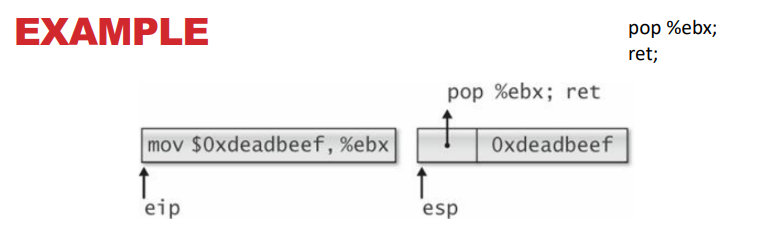
\includegraphics[width=13cm, keepaspectratio]{capitoli/secure_coding/img/cap_3/es_gadget.png}
    \caption{Esempio gadget.}\label{fig:es_gadget}
\end{figure}

Il gadget funziona nel seguente modo:
\begin{itemize}
    \item fa una pop del valore \verb|$0xdeadbeef| che si trova nello stack e lo inserisce nel registro ebx, facendo una pop viene diminuito anche la grandezza dello stack in base a quanto occupava quel valore in memoria. In questo caso si lavora con l'esp perchè si tiene conto della fine del frame che diminuisce;
    \item infine fa una ret che permette di eseguire il gadget successivo nello stack, come eip. Il nostro scopo è di creare una catena di gadget, composizione di varie operazioni, per l'attacco.
\end{itemize}

\paragraph{Esempio di attacco.}
L'obiettivo dell'attacco è di invocare la chiamata di sistema \\
\verb|ssize_t sys_write(unsigned int fd, const char * buf, size_t count)|
in modo da stampare a schermo “xxxHACKEDxxx”. Questa istruzione prende in input un \textit{file descriptor} in questo caso un stdout, una stringa e la dimensione della stringa da stampare.

\begin{figure}[H]
    \centering
    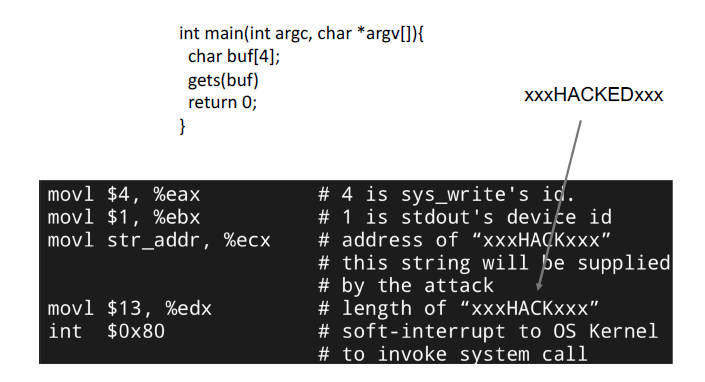
\includegraphics[width=13cm, keepaspectratio]{capitoli/secure_coding/img/cap_3/es_attacco_rop.png}
    \caption{Esempio attacco ROP.}\label{fig:es_attacco_rop}
\end{figure}
Vediamo nel dettaglio come funziona, per inserire il codice nello stack possiamo fare un buffer overflow come abbiamo visto nell'esempio del code injection:
\begin{enumerate}
    \item \verb|movl $4, %eax|: inserisce l'identificatore della sys\_write nel registro eax;
    \item \verb|movl $1, %ebx|: inserisce l'identificatore dello standard output stdout nel registro ebx;
    \item \verb|movl str_addr, %ecx|: copia l'indirizzo della stringa nel registro ecx;
    \item \verb|movl $13, %edx|: inserisce la grandezza della stringa nel registro edx, in questo modo abbiamo caricato nella CPU tutto quello che ci serve. Per prima mette la chiamata di sistema sys\_write e poi tutti i suoi parametri che abbiamo visto in precedenza;
    \item \verb|int $0x80|: int interrompe l'esecuzione della CPU e salta al valore salvato in eax che è 4 ovvero la funzione sys\_write.
\end{enumerate}
Proviamo a fare lo stesso attacco con i gadget.
\begin{figure}[H]
    \centering
    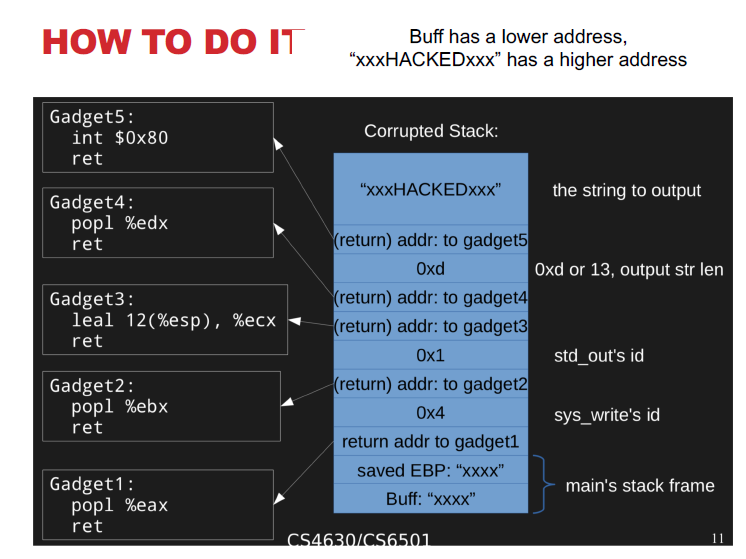
\includegraphics[width=13cm, keepaspectratio]{capitoli/secure_coding/img/cap_3/es_attacco_rop_gadget.png}
    \caption{Esempio attacco ROP con gadget.}\label{fig:es_attacco_rop_gadget}
\end{figure}

Nel caso di ROP, non c'è bisogno di scrivere un programma ma è necessario andare a trovare,
all'interno della \textbf{libc} ad esempio, dei gadget equivalenti alle istruzioni viste in precedenza.
Come si può vedere in Figura \ref{fig:es_attacco_rop_gadget} partendo dal basso verso l'alto dove il buff ha un indirizzo più basso rispetto
alla stringa “xxxHACKEDxxx”, abbiamo i primi due spazi di memoria dedicati al main frame con l'ebp e il buffer,
successivamente la prima istruzione da effettuare è la \textbf{ret} del Gadget1.
La ret permette di eliminare tutto quello che ci stava prima di "0x4" compreso il "return addr to gadget1" per poi passare a eseguire la prossima
istruzione del gadget1 che è \textbf{pop \%eax}.
Questa operazione è simile al funzionamento di eip ovvero esso contiene l'istruzione successiva da eseguire senza eliminare quello che è salvato prima.
Facendo la pop si elimina a sua volta quello che sta contenuto nella porzione di memoria successiva al return addr del gadget1 ovvero 0x4 e lo
inserisce nel registro eax. Si continua così per tutti gli altri gadget.
Nel Gadget3 si inserisce l'indirizzo di memoria della stringa che vogliamo stampare che è \textbf{12(\%esp)}
ovvero 12 byte sotto rispetto all'esp, il quale punta dopo la ret all'inizio di "return addr: to gadget 4".

\subsection{Qualche problema teorico}
In generale se il file eseguibile è più grande di 3 MB c'è una buona probabilità che si può trovare un insieme di gadget per ogni exploit, più il file è piccolo più diminuisce la probabilità di trovare dei gadget. Inoltre non è sempre necessario usare la ret ma possiamo usare anche il jump o altre, i ROP possono lavorare anche senza \textbf{libc} ma utilizzando il codice fornito. La tecnica ROP fornisce un  "linguaggio" (Turing complete) completamente funzionale che un utente malintenzionato può utilizzare
in modo da far eseguire  qualsiasi operazione desiderata a una macchina compromessa.

\subsection{Come si fa exploit/previene}
Il tool \textit{ROPgadget} è uno strumento automatizzato per aiutare ad automatizzare il processo di individuazione dei gadget e costruzione di un attacco contro un file binario. Esso ricerca all'interno del file binario dei potenziali gadget utili e tenta di assemblarli in un payload di attacco che produce una shell. Un altro modo semplice di creare un attacco ROP è tramite il framework CTF(Capture The Flag) \textbf{pwtools} \footnote{http://docs.pwntools.com/en/stable/rop/rop.html}, scritto in Python è stato progettato per la prototipazione rapida e per rendere la scrittura di exploit il più semplice possibile.


\newpage
\section{Forme di mitigazione}
Nella versione 4.1, GCC ha introdotto \textbf{Stack-Smashing Funzione Protector (SSP)}, che implementa i canarini derivati da StackGuard.

\subsection{Stack-Smashing Protector}
SSP o ProPolice è un estensione di GCC per la protezione delle applicazioni scritte in C dalle più comuni forme di exploit di buffer overflow. Esso riordina le variabili locali in modo da mettere i buffer dopo i puntatori e copia i puntatori che si trovano negli argomenti delle funzioni in un'area che precede i buffer delle variabili locali in modo da evitare la corruzione dei puntatori.

\subsection{I canarini}
I canarini consistono in un valore difficile da inserire o falsificare e sono scritti in un indirizzo prima della sezione di a pila da proteggere.  Di conseguenza, una scrittura sequenziale dovrebbe sovrascrivere questo valore per arrivare alla regione protetta.
\begin{figure}[H]
    \centering
    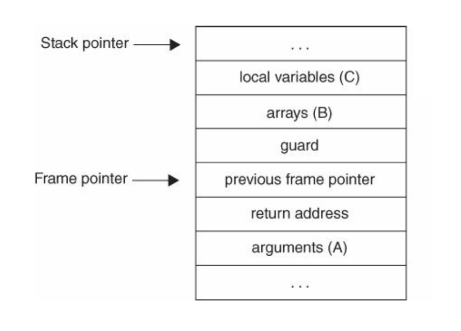
\includegraphics[width=12cm, keepaspectratio]{capitoli/secure_coding/img/cap_3/canarini.png}
    \caption{Canarino nello stack.}\label{fig:canarini}
\end{figure}
Come si può vedere in Figura \ref{fig:canarini}, il canarino viene inizializzato dopo che il return address è salvato ed è verificato
immediatamente prima di accedere a quest'ultimo. Un canarino casuale o difficile da falsificare è un numero casuale segreto a 32-bit che cambia ogni
volta che il programma viene eseguito. Le opzioni \verb|-fstack-protector| e \verb|-fno-stack-protector| abilitano o disabilitano SSP per la protezione di
oggetti vulnerabili.

\subsection{Address Space Layout Randomization}
L' ASLR è una caratteristica della sicurezza di molti sistemi operativi, il suo scopo è di evitare l'esecuzione di codice arbitrario. Essa permette di randomizzare gli indirizzi delle pagine di memoria usate dal programma. Però ASLR non previene la sovrascrittura del return address da parte di un overflow basato sullo stack. In ogni caso esso potrebbe prevenire la predizione corretta da parte degli attaccanti dell'indirizzo dello shellcode, delle funzioni di sistema dei gadget ROP che vogliono invocare.

\subsection{Stack non-eseguibile}
Uno stack non eseguibile è una soluzione runtime (a tempo di esecuzione) che è stata progettata per prevenire l'esecuzione di codice eseguibile  nel segmento dello stack. Esso previene il buffer overflow solo sullo stack non sull'heap, inoltre non prevengono il fatto di poter usare l'overflow per un modificare un indirizzo di ritorno, un puntatore ad un oggetto o ad una funzione. Non prevengono la code o arc injection o la ROP.

\subsection{W xor X}
Molti sistemi operativi, come OpenBDS, Windows, Linux e OS X, impone privilegi ridotti nel kernel così
che nessuna parte dello spazio degli indirizzi del processo è sia scrivibile che eseguibile.
Questa politica è chiamata W xor X (W$\bigoplus$X) ed è supportato dall'uso di un bit No eXecute (NX) attivo diverse CPU.